\documentclass{article}
\usepackage{graphicx}
\usepackage[margin=1in]{geometry}
\usepackage[outdir=./]{epstopdf}  					% Avoids errors when input figures
\usepackage[labelsep=period,labelfont=bf]{caption}
%\usepackage{subcaption}

\begin{document}
	\begin{figure}[tbph]
		\caption{Response of the Forward Premium to U.S. Monetary Policy Surprises} \label{fig:LPEMRHO}
		\begin{center}
			\begin{minipage}{\linewidth}
				\begin{center}
					\begin{subfigure}[t]{\linewidth}
						\includegraphics[trim={0cm 0cm 0cm 0cm},clip,height=0.235\textheight,width=\linewidth]{../Figures/LPs/LagDep-FX/Target/EM/TargetEMrho.eps} \\
						\vspace{-0.35cm}
						\caption{Target Surprise: 2000-2008} \label{subfig:LPEMRHOtarget}
%						\vspace{0.4cm}
					\end{subfigure}
					
					\begin{subfigure}[t]{\linewidth}
						\includegraphics[trim={0cm 0cm 0cm 0cm},clip,height=0.235\textheight,width=\linewidth]{../Figures/LPs/LagDep-FX/Path/EM/PathEMrho.eps} \\
						\vspace{-0.35cm}
						\caption{Forward Guidance Surprise: 2000-2019} \label{subfig:LPEMRHOpath}
					\end{subfigure}
					
					\begin{subfigure}[t]{\linewidth}
						\includegraphics[trim={0cm 0cm 0cm 0cm},clip,height=0.235\textheight,width=\linewidth]{../Figures/LPs/LagDep-FX/LSAP/EM/LSAPEMrho.eps} \\
						\vspace{-0.35cm}
						\caption{Asset Purchase Surprise: 2009-2019} \label{subfig:LPEMRHOlsap}
					\end{subfigure}
				\end{center}
				\fignotes{This figure shows the response following \cite{Jorda:2005} of the 10- and 2-year foreign exchange forward premium of emerging markets to easing surprises in U.S. monetary policy of 1 basis point. The forward premium is calculated using cross-currency swaps, which are in turn constructed using cross-currency basis swaps and interest rate swaps, see section \ref{sec:YCsynt} for details. The target, forward guidance and asset purchase surprises are identified using intraday data around Fed's monetary policy announcements, see section \ref{sec:USMPS} for details. An arrow indicates the contemporaneous (\(\idxh = 0\)) effect. The 90\% confidence bands are based on Driscoll--Kraay standard errors.}
			\end{minipage}
		\end{center}
	\end{figure}
\end{document}
% trim = {<left> <lower> <right> <upper>}